\documentclass[12pt]{article}
\usepackage[margin=1in]{geometry}
\usepackage{amsmath, amsthm, amssymb, amsfonts, enumitem, graphicx}
\usepackage{fancyhdr}

\theoremstyle{definition}
\newtheorem{problem}{Problem}
\renewcommand*{\proofname}{Solution}
\renewcommand{\theenumi}{\alph{enumi}}

\newcommand{\vect}[1]{\boldsymbol{#1}}

\newenvironment{amatrix}[1]{%
  \left[\begin{array}{@{}*{#1}{c}|c@{}}
}{%
  \end{array}\right]
}

\newcommand{\grstep}[2][\relax]{%
   \ensuremath{\mathrel{
       {\mathop{\longrightarrow}\limits^{#2\mathstrut}_{
                                     \begin{subarray}{l} #1 \end{subarray}}}}}}
\newcommand{\swap}{\leftrightarrow}

\pagestyle{fancy}
\fancyhf{}
\rhead{Homework Assignment 2}
\lhead{Matthew Tiger}
\cfoot{\thepage}


\title{Homework Assignment 2}
\author{Matthew Tiger}


\begin{document}


\maketitle


% Problem 1
\begin{problem}
  Convert the following linear programming problem to \textit{standard form}:
  \begin{align*}
    \begin{array}{rll}
      \text{maximize} & 2x_1 + x_2 &\\
      \text{subject to} & 0 \leq x_1 &\leq 2 \\
      & x_1 + x_2 &\leq 3 \\
      & x_1 + 2x_2 &\leq 5 \\
      & x_2 \geq 0 &
    \end{array}
  \end{align*}
\end{problem}

\begin{proof}
  In order to convert this linear programming problem into standard form, we
  must transform the objective from \textit{maximize} to \textit{minimize} and
  the constraints must be transformed from linear inequalities into linear equations.

  Our first step will be to rewrite the objective function as a minimization problem
  and write each constraint as a linear inequality as so:
  \begin{align*}
    \begin{array}{rll}
      \text{minimize} & -2x_1 - x_2 &\\
      \text{subject to} & x_1 &\leq 2 \\
      & x_1 + x_2 &\leq 3 \\
      & x_1 + 2x_2 &\leq 5 \\
      & x_1 \geq 0, x_2 \geq 0 &
    \end{array}
  \end{align*}

  We can then introduce three slack variables $x_3, x_4, x_5$ to turn the linear
  inequalities into linear equations:
  \begin{align*}
    \begin{array}{rllllll}
      \text{minimize} & -2x_1 &- x_2  & & & &\\
      % \text{subject to} & x_1 & &+ x_3 & & &= 2 \\
      \text{subject to} & x_1 &+ x_2 &+ x_3 & & &= 2 \\
      & x_1 &+ x_2 & &+ x_4 & &= 3 \\
      & x_1 &+ 2x_2 & & &+ x_5&= 5 \\
      & x_1 \geq 0, &x_2 \geq 0, &x_3 \geq 0, &x_4 \geq 0, &x_5 \geq 0
    \end{array}
  \end{align*}

  As the above linear programming problem is written as
  \begin{align*}
    \begin{array}{rl}
      \text{minimize} & \vect{c}^\intercal \vect{x}\\
      \text{subject to} & A\vect{x} = \vect{b} \\
      & \vect{x} \geq 0
    \end{array}
  \end{align*}
  where
  \begin{align*}
    \vect{c}^\intercal =
    \begin{bmatrix}
      -2 \\
      -1 \\
    \end{bmatrix}^\intercal,
    \quad
    A =
    \begin{bmatrix}
      1 & 1 & 1 & 0 & 0 \\
      1 & 1 & 0 & 1 & 0 \\
      1 & 2 & 0 & 0 & 1 \\
    \end{bmatrix},\quad
    \vect{x} =
    \begin{bmatrix}
      x_1 \\
      x_2 \\
      x_3 \\
      x_4 \\
      x_5 \\
    \end{bmatrix}, \quad
    \vect{b} =
    \begin{bmatrix}
      2 \\
      3 \\
      5 \\
    \end{bmatrix}
  \end{align*}
  with $\vect{x} \geq 0$ and $\vect{b} \geq 0$ the linear programming problem
  is in standard form and we are done.
\end{proof}
\newpage


% Problem 2
\begin{problem}
  Solve the system $A\vect{x} = \vect{b}$ where
  \begin{align*}
    A =
    \begin{bmatrix}
      2 & -1 & 2 & -1 & 3 \\
      1 & 2 & 3 & 1 & 0 \\
      1 & 0 & -2 & 0 & -5 \\
    \end{bmatrix}
    , \quad
    \vect{b} = \begin{bmatrix}
      14 \\
      5 \\
      -10 \\
    \end{bmatrix}.
  \end{align*}
  If possible, generate a non-basic feasible solution of the system from which
  you derive next a basic feasible one.
\end{problem}

\begin{proof}
  In order to solve the system $Ax=b$, we must perform row operations on the
  augmented matrix to reduce it to reduced row form. We perform these operations below:

  \begin{align*}
    &\begin{amatrix}{5}
      2 & -1 & 2 & -1 & 3 & 14 \\
      1 & 2 & 3 & 1 & 0 & 5 \\
      1 & 0 & -2 & 0 & -5 & -10 \\
    \end{amatrix}
    \begin{array}{c}
    \grstep[{[2] - (1/2)[1]}]{(1/2)[1]} \\
    \grstep[]{[3] - (1/2)[1]}
    \end{array}
    \begin{amatrix}{5}
      1 & -1/2 & 1 & -1/2 & 3/2 & 7 \\
      0 & 5/2 & 2 & 3/2 & -3/2 & -2 \\
      0 & 1/2 & -3 & 1/2 & -13/2 & -17 \\
    \end{amatrix}
    \begin{array}{c}
      \grstep[]{(2/5)[2]}
    \end{array}
    \\
    &\begin{amatrix}{5}
      1 & -1/2 & 1 & -1/2 & 3/2 & 7 \\
      0 & 1 & 4/5 & 3/5 & -3/5 & -4/5 \\
      0 & 1/2 & -3 & 1/2 & -13/2 & -17 \\
    \end{amatrix}
    \begin{array}{c}
      \grstep[{[3] - (1/2)[2]}]{[1] + (1/2)[2]} \\
    \end{array}
    \begin{amatrix}{5}
      1 & 0 & 7/5 & -1/5 & 6/5 & 33/5 \\
      0 & 1 & 4/5 & 3/5 & -3/5 & -4/5 \\
      0 & 0 & -17/5 & 1/5 & -31/5 & -83/5 \\
    \end{amatrix}
    \\
    &\begin{array}{c}
      \grstep[]{(-5/17)[3]}
    \end{array}
    \begin{amatrix}{5}
      1 & 0 & 7/5 & -1/5 & 6/5 & 33/5 \\
      0 & 1 & 4/5 & 3/5 & -3/5 & -4/5 \\
      0 & 0 & 1 & -1/17 & 31/17 & 83/17 \\
    \end{amatrix}
    \begin{array}{c}
      \grstep[{[2] - (4/5)[3]}]{[1] - (7/5)[3]} \\
    \end{array}
    \begin{amatrix}{5}
      1 & 0 & 0 & -2/17 & -23/17 & -4/17 \\
      0 & 1 & 0 & 11/17 & -35/17 & -80/17 \\
      0 & 0 & 1 & -1/17 & 31/17 & 83/17 \\
    \end{amatrix}.
  \end{align*}

  Using the above row-reduced augmented matrix, we see that the solution to the
  system $A\vect{x} = \vect{b}$ is given by
  \begin{align}\label{prob_2_x}
    \vect{x} =
    \begin{bmatrix}
      -4/17 \\
      -80/17 \\
      83/17 \\
      0 \\
      0 \\
    \end{bmatrix}
    +
    s
    \begin{bmatrix}
      2/17 \\
      -11/17 \\
      1/17 \\
      1 \\
      0 \\
    \end{bmatrix}
    +
    t
    \begin{bmatrix}
      23/17 \\
      35/17 \\
      -31/17 \\
      0 \\
      1 \\
    \end{bmatrix}
  \end{align}
  where $s\in\mathbb{R}$ and $t\in\mathbb{R}$.

  Suppose that the matrix $A$ is written such that $A = [\vect{a}_i]$ for
  $1 \leq i \leq 5$ where $\vect{a}_i$ corresponds to the $i$-th column of the original
  matrix $A$. Recall that a solution $\vect{x}_0 \geq \vect{0}$ of the system $A\vect{x} = \vect{b}$ is a
  basic feasible solution if the columns of the matrix
  $A$ associated to the nonzero components of $\vect{x}_0$ are linearly
  independent. Otherwise the solution is a non-basic feasible solution.

  Using solution \eqref{prob_2_x}, we see that for $s = 0$ and $t = 82/31$, we get
  the corresponding feasible solution $\vect{x}_0 = [1762/527, 390/527, 1/17, 0, 82/31]^\intercal$ to the system
  $A\vect{x} = \vect{b}$. We know that this is a non-basic feasible solution since the vectors
  $\vect{a}_1$, $\vect{a}_2$, $\vect{a}_3$, and $\vect{a}_5$ must be linearly
  dependent as the $\text{rank}(A) = 3$, i.e.\ the maximum number of linearly independent columns of $A$ is 3.

  The Fundamental Theorem of LP prescribes how to move from this non-basic feasible
  solution $\vect{x}_0$ to a basic feasible solution $\vect{x}_1$. As $\vect{a}_1$, $\vect{a}_2$, $\vect{a}_3$, and $\vect{a}_5$
  are linearly dependent, there exists constants $y_1, y_2, y_3, y_5$ not all zero such that
  \begin{align*}
    y_1\vect{a_1} + y_2\vect{a_2} + y_3\vect{a_3} + y_5\vect{a_5} = \vect{0},
  \end{align*}
  namely $y_1 = 1$, $y_2 = 35/23$, $y_3 = -31/23$, and $y_5 = 17/23$.
  Thus, the vector $\epsilon\vect{y} = \epsilon[y_1, y_2, y_3, 0, y_5] ^ \intercal$ satisfies
  $A[\epsilon\vect{y}] = \vect{0}$. As such, the vector $\vect{x}_0 - \epsilon\vect{y}$ satisfies
  $A[\vect{x}_0 - \epsilon\vect{y}] = \vect{b}$, i.e.\ the vector $\vect{x}_0 - \epsilon\vect{y}$
  is a solution of the original system $A\vect{x} = \vect{b}$. Choose
  $$\epsilon = \min\{x_i/y_i| i=1,2,3,5\ y_i > 0\} = -23/527.$$
  Then the vector $\vect{x}_1 = \vect{x}_0 - \epsilon\vect{y}$ will have 3 positive components and the rest of the components will be 0 showing that
  the vector $\vect{x}_1$ is a basic feasible solution. Therefore,
  \begin{align*}
    \vect{x}_1 = \vect{x}_0 - \epsilon\vect{y} = \begin{bmatrix}105/31\\ 25/31\\ 0\\ 0\\ 83/31\end{bmatrix}
  \end{align*}
  is the desired basic feasible solution.
\end{proof}
\newpage


% Problem 3
\begin{problem}
  Does every linear programming problem in standard form have a nonempty feasible set?
  If ``yes'', provide a proof. If ``no'', provide a counter-example.

  Does every linear programming problem in standard form (assuming a nonempty feasible
  set) have an optimal solution? If ``yes'', provide a proof. If ``no'', provide a counter-example.
\end{problem}

\begin{proof}
  Not every linear programming problem (LP) in standard form has a nonempty feasible set.
  Take for instance the following LP:
  \begin{align*}
    \begin{array}{rl}
      \text{minimize} & 2x_1 \\
      \text{subject to} & x_1 \leq -1 \\
      & x_1 \geq 0
    \end{array}
  \end{align*}
  Clearly this problem has an empty feasible set due to the contradictory constraints.

  The LP in standard form is stated as:
  \begin{align*}
    \begin{array}{rl}
      \text{minimize} & 2x_1  \\
      \text{subject to} & -x_1 - x_2  = 1  \\
      & x_1 \geq 0,  x_2 \geq 0
    \end{array}
  \end{align*}
  The equation $-x_1 - x_2 = 1$ for $x_1, x_2 \geq 0$ has no solutions
  and the feasible set of the standard form LP is empty.
  Therefore, not every LP in standard form has a nonempty feasible set.

  Additionally, not every LP in standard form with a nonempty feasible set has
  an optimal solution. Take for instance the following LP:
  \begin{align*}
    \begin{array}{rl}
      \text{minimize} & -3x_1 \\
      \text{subject to} & x_1 \geq 1  \\
      & x_1 \geq 0
    \end{array}
  \end{align*}
  The problem can be written in standard form as so:
  \begin{align*}
    \begin{array}{rl}
      \text{minimize} & -3x_1  \\
      \text{subject to} & x_1 - x_2 = 1  \\
      & x_1 \geq 0, x_2 \geq 0
    \end{array}
  \end{align*}
  The equation $x_1 - x_2 = 1$ for $x_1, x_2 \geq 0$ has an infinite number of
  solutions so that $x_1$ can be chosen arbitrarily large. Consequently,
  $-x_1$ can be made arbitrarily small and no point in
  the feasible set of this LP in standard form is the smallest, i.e\ optimal.
  Therefore, not every LP in standard form with a nonempty feasible set has an optimal solution.
\end{proof}
\newpage


% Problem 4
\begin{problem}
  \begin{enumerate}
    \item Solve the following linear program graphically:
      \begin{align*}
        \begin{array}{ll}
          \text{maximize} & 2x_1 + 5x_2 \\
          \text{subject to} & 0 \leq x_1 \leq 4 \\
          & 0 \leq x_2 \leq 6 \\
          & x_1 + x_2 \leq 8
        \end{array}
      \end{align*}
    \item Solve the linear program in (b) the same way Example 15.15 was solved in class.
      Compute only the vertices that lead to the optimal vertex found at (a).
  \end{enumerate}
\end{problem}

\begin{proof}
  \begin{enumerate}
    \item In order to find the solution to this linear program, we must first
      plot the feasible region of this problem. Note, that the equation associated
      to the objective function forms a family of straight lines $O = \{2x_1 + 5x_2 = b\ |\ b\in \mathbb{R}\}$.
      We then wish to find a value $b$ such that the line $2x_1 + 5x_2 = b$ is within the
      feasible region, i.e.\ satisfies the constraints and the value $b$ is the
      largest such value that allows $x_1$ and $x_2$ to satisfy the constraints.

      After plotting the feasible region with Mathematica and trying various values of $b$,
      we see that an objective function value $b=34$ is associated to the optimal solution of this LP
      as the plot below shows:
      \begin{figure}[!h]
        \centerline{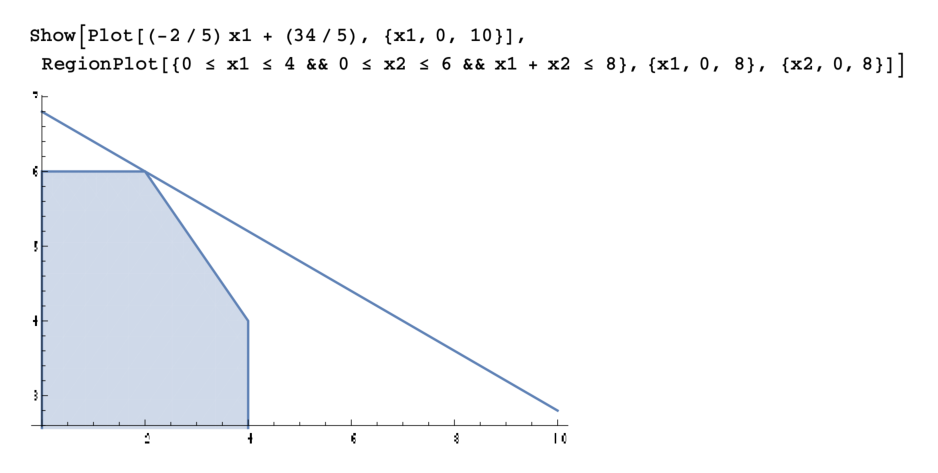
\includegraphics[scale=0.9]{geometric_solution}}
      \end{figure}

      It is easy to see that any $b > 34$ will cause the objective function to
      leave the feasible region, providing a geometric proof that $(x_1, x_2) = (2, 6)$
      is the optimal solution of this linear program leading to an optimal objective
      function value of $34$.
    \item In order to solve this problem, we must first transform the problem into
      standard form through the addition of slack variables and changing the
      objective as follows:
      \begin{align*}
        \begin{array}{rllllll}
          \text{minimize} & -2x_1 &-5x_2 & & & &\\
          \text{subject to} & x_1 & &+ x_3& & &= 4 \\
          & & \phantom{+}x_2 & &+ x_4 & &= 6 \\
          & x_1 &+ x_2& &  &+ x_5 &= 8 \\
          &x_1, &x_2, &x_3, &x_4, &x_5 &\geq 0
        \end{array}.
      \end{align*}

      In matrix form, this linear program is represented as
      \begin{align*}
        \begin{array}{rl}
          \text{minimize} & \vect{c}^\intercal \vect{x} = [-2, 5, 0, 0, 0] [x_1, x_2, x_3, x_4, x_5]^\intercal \\
          \text{subject to} & A\vect{x} =
          \begin{bmatrix}
            1 & 0 & 1 & 0 & 0\\
            0 & 1 & 0 & 1 & 0\\
            1 & 1 & 0 & 0 & 1\\
          \end{bmatrix}
          \begin{bmatrix}
            x_1 \\
            x_2 \\
            x_3 \\
            x_4 \\
            x_5 \\
          \end{bmatrix} =
          \begin{bmatrix}
            4 \\
            6 \\
            8 \\
          \end{bmatrix} = \vect{b} \\
          & \vect{x} \geq 0
        \end{array}.
      \end{align*}
    Note that we can represent the matrix $A$ in terms of its columns as follows:
    \begin{align*}
      A =
      \begin{bmatrix}
        1 & 0 & 1 & 0 & 0\\
        0 & 1 & 0 & 1 & 0\\
        1 & 1 & 0 & 0 & 1\\
      \end{bmatrix}
      =
      \begin{bmatrix}
        \vect{a_1}
        \vect{a_2}
        \vect{a_3}
        \vect{a_4}
        \vect{a_5}
      \end{bmatrix}.
    \end{align*}

    We begin by finding a basic feasible solution of the system. In order to find the optimal value for this linear program, we will move from
    this basic feasible solution to an adjacent basic feasible solution. We keep moving
    to adjacent basic feasible solutions until the objective function does not decrease any further.
    The solution at which this occurs will be optimal.

    Note that
    $\vect{x} = [0, 0, 4, 6, 8]^\intercal$ is a basic feasible
    solution as $\vect{a_3}, \vect{a_4}, \vect{a_5}$ are linearly independent and $\vect{x} \geq 0$.
    The objective function's value for this basic feasible solution is $\vect{c}^\intercal \vect{x} = 0$.

    To choose an adjacent basic feasible solution, we choose $\vect{a_2}$ as a basic
    column in the new basis. We can express $\vect{a_2}$ as a linear combination
    of the old basic columns $\vect{a_3}, \vect{a_4}, \vect{a_5}$:
    \begin{align*}
      \vect{a_2} = 0\vect{a_3} + 1\vect{a_4} + 1\vect{a_5}.
    \end{align*}
    We now wish to find an $\epsilon > 0$ such that
    \begin{align*}
      0\vect{a_1} + \epsilon\vect{a_2} + (4 - 0\epsilon)\vect{a_3} + (6-1\epsilon)\vect{a_4} + (8-1\epsilon)\vect{a_5} = \vect{b}
    \end{align*}
    and the coefficients of the above system are non-negative while also eliminating
    either $\vect{a_3}, \vect{a_4}, \vect{a_5}$. The choice of $\epsilon = 6$ satisfies the
    above requirements leading to the new basic feasible solution
    \begin{align*}
      \vect{x} = [0, 6, 4, 0, 2]^\intercal.
    \end{align*}

    We now repeat the procedure choosing to make $\vect{a_1}$ the new basic
    column. We write $\vect{a_1}$ as a linear combination of the basic columns
    $\vect{a_2}, \vect{a_4}, \vect{a_5}$ as follows:
    \begin{align*}
      \vect{a_1} = 0\vect{a_2} + 1\vect{a_3} + 1\vect{a_5}.
    \end{align*}
    We now need to find $\epsilon > 0$ such that
    \begin{align*}
      \epsilon\vect{a_1} + (6-0\epsilon)\vect{a_2} + (4-1\epsilon)\vect{a_3} + 0\vect{a_4} + (2-1\epsilon)\vect{a_5} = \vect{b}
    \end{align*}
    that maintains the non-negativity of the solution and eliminates either $\vect{a_2}, \vect{a_3}$, or $\vect{a_5}$.
    The choice of $\epsilon = 2$ satisfies these requirements leading us to the new
    basic feasible solution
    \begin{align}\label{basic_solution}
      \vect{x} = [2, 6, 2, 0, 0]^\intercal
    \end{align}
    Choosing either $\vect{a_4}$ or $\vect{a_5}$ to be the new basic columns will
    reduce the value of $x_1$ or $x_2$ in \eqref{basic_solution} thereby leading to an objective function value greater than the current one. This would mean that the next solution
    could not be optimal. Therefore,
    \eqref{basic_solution} is the optimal solution to the linear program with
    associated objective function value -34, or 34 in terms of the objective
    function of the original linear program.
  \end{enumerate}
\end{proof}

\end{document}
